%!TEX root = TIWSNE_Mini_project_main.tex
\section{Image}

The test image was received correctly on the PC. 
The result can be seen in figure \ref{fig:compressedlena}.

\begin{figure}[H]
\centering
\begin{subfigure}{.5\textwidth}
  \centering
  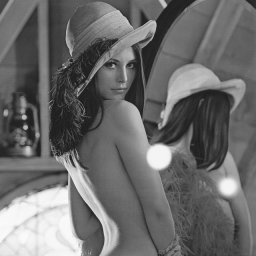
\includegraphics[width=.6\linewidth]{lena}
  \caption{The original, uncompressed test image.}
  \label{fig:lena}
\end{subfigure}%
\begin{subfigure}{.5\textwidth}
  \centering
  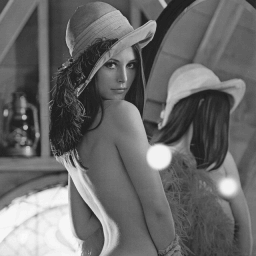
\includegraphics[width=.6\linewidth]{lenacompressed2bit}
  \caption{The test image after being  compressed - 2 least significant bits truncated.}
  \label{fig:compressedlena}
\end{subfigure}
\caption{The test image with and without compression.}
\label{fig:lenacomp}
\end{figure}

As can be seen on figure \ref{fig:lenacomp}, the image resulting from the simple truncation compression is not visibly different from the original image, without a thorough comparison. 
Thus the reduction in image quality has not been detrimental.

The correctness of the compression was verified by studying the content of the file before and after compression. 
A comparison of the two files is shown in figure \ref{fig:hexlenacomp}. 

\begin{figure}[H]
\centering
\begin{subfigure}{.5\textwidth}
  \centering
  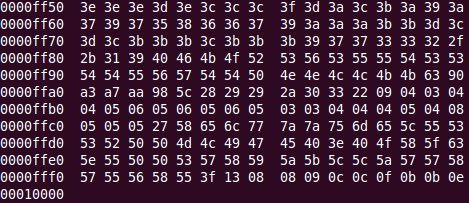
\includegraphics[width=0.95\linewidth]{rawhexdump}
  \caption{Hexdump of the original image.}
  \label{fig:lenahex}
\end{subfigure}%
\begin{subfigure}{.5\textwidth}
  \centering
  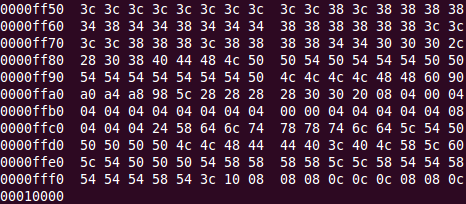
\includegraphics[width=0.95\linewidth]{compressedhexdump}
  \caption{Hexdump of the compressed image.}
  \label{fig:compressedlenahex}
\end{subfigure}
\caption{Content of the image file with and without compression.}
\label{fig:hexlenacomp}
\end{figure}

%discussion: harder compression